\section{Fachkonzept}
In diesem Kapitel werden die im Projekt eingesetzten Technologien beschrieben.\\
\begin{figure}[h]
    \centering
    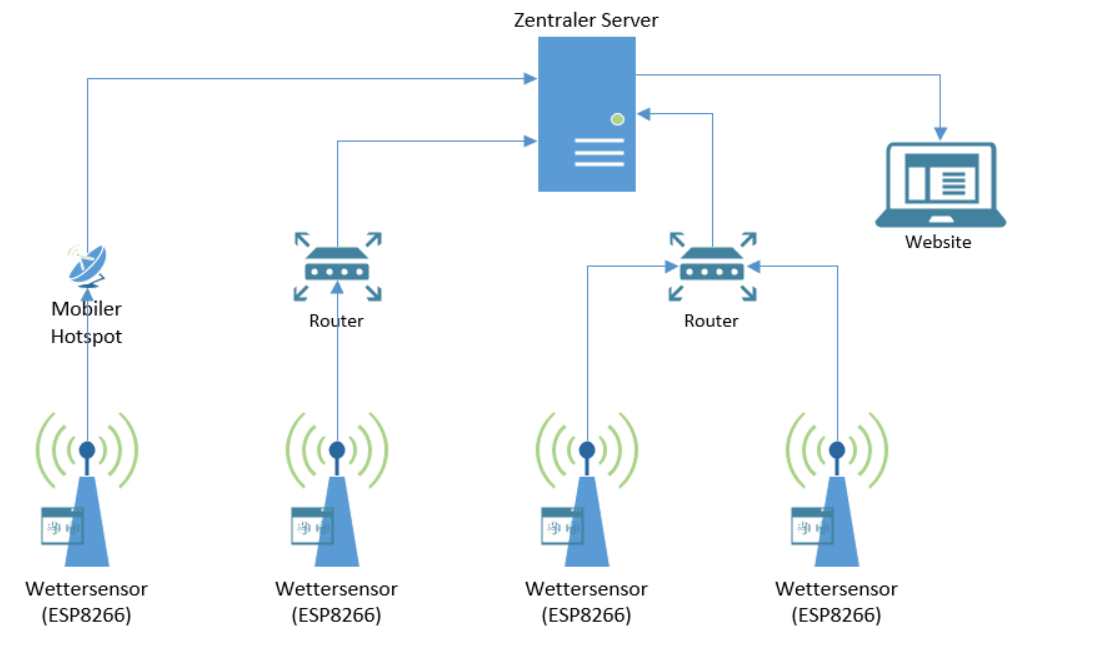
\includegraphics[width=0.7\linewidth]{img/projektkomponenten}
    \caption[Komponenten des Gesamtsystems]{Komponenten des Gesamtsystems (eigene Darstellung)}
    \label{fig:projektkomponenten}
\end{figure}
\\
In \autoref{fig:projektkomponenten} ist ein möglicher Aufbau der Projektkomponenten gemäß den Projektanforderungen\footnote{\cite{Wortmann.2020}} dargestellt.

\subsection{Mikrocontroller}
Wie in \autoref{ESP} beschrieben, kommt im Projekt ein ESP8266 Mikrocontroller zum Einsatz. Auf dem Mikrocontroller erfolgt die Erfassung der Messdaten mit einem BME280-Sensor und der Versand an das Backend.
Bei der Auswahl der Libraries wurde hierbei beachtet, möglichst auf den Anwendungsfall spezifische Libraries zu wählen um die Auslastung des Mikrocontrollers zu minimieren.
Ein geringer Energieverbrauch wird in der Programmierung besonders beachtet. Dadurch ist die Funktionalität auf das wesentliche beschränkt während trotzdem eine zuverlässige Funktionsweise gewährleistet wird. Wenn der Mikrocontroller keine Verbindung zum angegebenen WLAN-Netzwerk herstellen kann oder der Server nicht erreichbar ist, werden die Daten gecached und versandt, sobald eine Verbindung hergestellt werden kann.\\
Der Mikrocontroller wird in der Arduino IDE in C++ programmiert.

\subsection{Zentraler Server}
Auf dem zentralen Server wird das Backend des Projekts bereitgestellt. Das Backend ist in JavaScript geschrieben und verwendet eine SQLite-Datenbank für die Speicherung der Daten. Für die Kommunikation zu den Sensoren und dem Frontend ist eine REST-API vorhanden, die in \autoref{Schnittstellen} näher erläutert wird.\\
Das Projekt nutzt node.js Version 14.4 und SQLite-Version 3.\\
Sowohl das Backend als auch das Frontend sind für das Deployment in Docker vorgesehen. Hierbei ist eine örtliche Trennung möglich, das Frontend kann auf jeden Server zugreifen, der die API dieses Projekts bereitstellt.

\subsection{Website}
Die Website basiert ebenfalls auf JavaScript für die Logik. Aufgrund des Projektaufbaus ist es wie oben genannt möglich, das Hosting von Backend und Frontend zu trennen.\\
Für die Bereitstellung des Frontends kommen einige Node-Libraries zum Einsatz. Die Darstellung der Messdaten auf der Website erfolgt mit Chart.js\footnote{\cite{chartjs.2020}}. Die Auswahl eines Zeitraums für die Darstellung eines Intervalls ist mit der Library daterangepicker\footnote{\cite{daterangepicker.2020}} umgesetzt.
Die HTML- und CSS-Komponenten der Website sind mit Bootstrap 4 erstellt worden. Auf die Gestaltung wird in \autoref{GUI-Konzept} näher eingegangen.